% !TeX spellcheck = de_DE
\documentclass{alex_gp}

\name{Alexander Helbok}
\course{Grundpraktikum}
\hwnumber{3}
\spacing{}

\begin{document}
\renewcommand{\labelenumi}{\alph{enumi})}


\begin{mybox}{Eine Feder mit drei Massen}
	Um die Masse des Pendelkörpers zu bestimmen, wurde das IOLab an einer Schnur aus der Ruhelage hochgezogen. Dabei wurde die Beschleunigung und die Kraft in vertikaler Richtung gemessen und nach Newtons zweitem Axiom gilt dann für die Masse
	\begin{equation}\label{eqn:newt}
		m = \tfrac{F}{a} 
	\end{equation}
	Für die gemessene Beschleunigung \( a \) wird ein Fehler von \( 0.001 \unit{\a} \) angenommen, da das die Genauigkeit ist, mit der die Beschleunigung im Programm angegeben wird. Der Kraft \( F \) wird ein Fehler von \( 0.0025 \unit{N} \) zugesprochen, weil der Sensor ein Auflösungsvermögen von \( 0.005 \unit{N} \) hat. In Abbildung \ref{fig:mass} ist die Bestimmung der einer Masse (Dritten und Schwersten) dargestellt.
	\begin{figure}[H]
		\vspace{-1cm}		
		\centering
		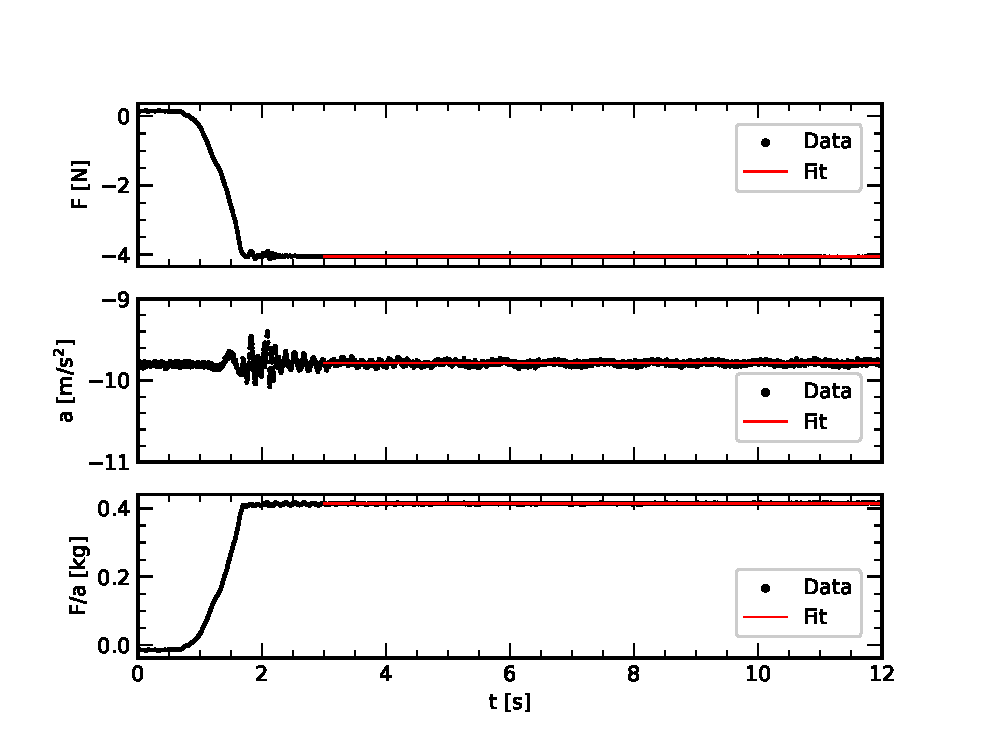
\includegraphics[width=\textwidth]{Versuch3_1.eps}
		\caption{Vom oben nach unten sind Kraft \( F \), Beschleunigung \( a \) und die Masse als Quotient zwischen Kraft und Beschleunigung \( F/a \) aufgetragen. Die Drei Grafiken teilen sich die horizontale Achse. Zudem sind in Rot Geraden von \( t = 3 \unit{s} \) bis \( t = 12 \unit{s} \) angepasst.}
		\label{fig:mass}
	\end{figure}
	
	Hängt man das IOLab an eine Feder und lenkt diese aus, fängt das System an zu Pendeln. Diese Schwingungen lassen sich mittels Beschleunigungs- und/oder Kraftsensors aufzeichnen und aus ihnen kann man charakteristische Eigenschaften der Oszillation, wie die Schwingungsdauer \( T \) oder die Kreisfrequenz \( \omega \), bestimmen. Dafür wurde eine Sinuskurve mit einem Fitprogramm an die Messpunkte angepasst, wobei die an SciPy übergebenen Daten nur „schöne“ Schwingungen enthalten.\par 
	
	Für die Analyse der Schwingungsdaten wurde der Beschleunigungssensor verwendet, da dieser ein höheres Auflösungsvermögen als der Kraftsensor hat. In Abbildung \ref{fig:sine} sieht man eine an die Beschleunigungsdaten angepasste Sinuskurve. Die Amplituden stimmen nicht ganz überein, da die Maxima und Minima aufgrund von Reibung und Luftwiderstand mit der Zeit abnehmen und dies im Sinusfit nicht berücksichtigt wird. Die Amplitude der angepassten Kurve kann man sich als den Mittelwert aller Maxima vorstellen und ist daher zu Beginn der Messung etwas zu Niedrig und gegen Ende zu Groß.
	
	\begin{figure}[H]
		\vspace{-1cm}		
		\centering
		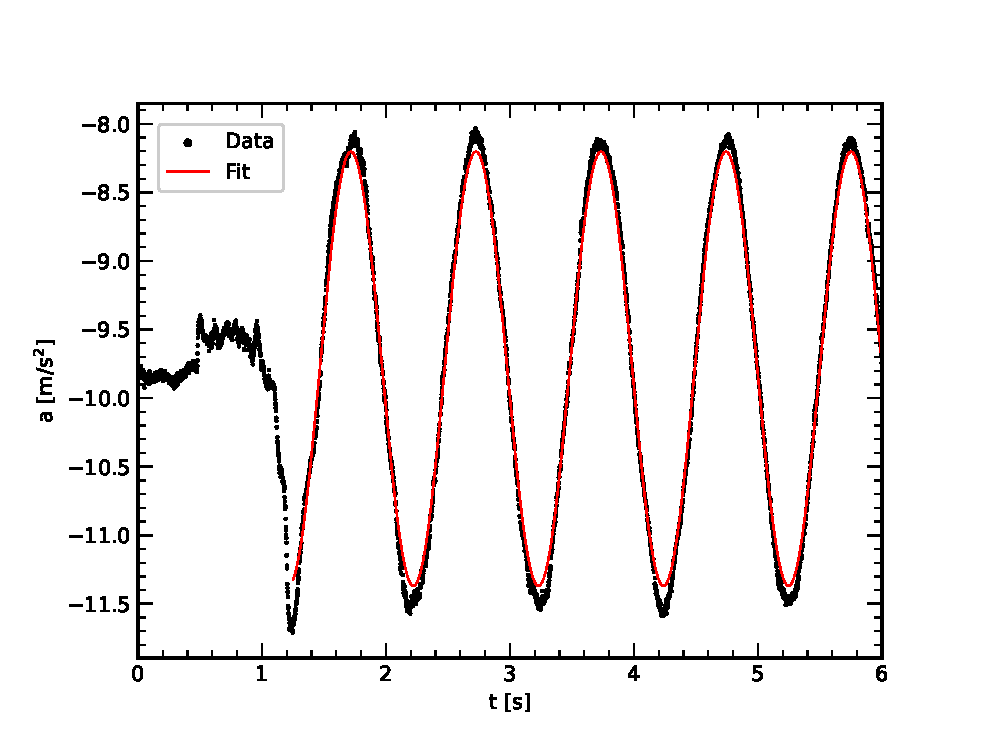
\includegraphics[width=\textwidth]{Versuch3_2.eps}
		\caption{Die Beschleunigung wurde auf die Zeit aufgetragen und eine Sinuskurve in Rot wurde an die Daten ab \( t = 1 \unit{s} \) (bis \( t = 40 \unit{s} \)) angepasst.}
		\label{fig:sine}
	\end{figure}
	
	Es wurden 3 Versuche mit unterschiedlichen Massen und gleicher Feder durchgeführt.In Tabelle \ref{table:1} sind Masse, Wurzel der Kehrwerts der Masse, Periode und Winkelfrequenz der verschiedenen Versuche mit dazugehörigen Fehlern aufgelistet. \par
	\centering
	\begin{tabular}{@{}r c r c r c r @{}}\toprule
		&& Versuch1 && Versuch 2 && Versuch 3 \\ \midrule
		\( m \) [kg] && 0.202() && 0.355() && 0.414() \\
		\( \sqrt{1/m}\; [\text{kg}^{-\tfrac{1}{2}}] \) && 2.220() && 1.677() && 1.553() \\
		T [s] && 1.509() && 1.867() && 2.016() \\
		$\omega$ [s\( ^{-\tfrac{1}{2}} \)] && 8.326() && 6.729() && 6.232() \\
		\bottomrule
	\end{tabular}
	\captionof{table}{Gemessene Masse, Schwingungsdauer und Winkelfrequenz der drei Versuche}
	\label{table:1}
	
	
\end{mybox}

\begin{mybox}{Entwicklung eines Modells für parallele Federn}
	\begin{tabular}{@{}r | r @{}}\toprule
		N & \( \omega [\text{s}^{-1}]\) \\ \midrule
		1 & 16.115() \\
		2 & 31.664() \\
		3 & 46.614() \\
		\bottomrule
	\end{tabular}
\end{mybox}

\begin{mybox}{}

\end{mybox}


\end{document}